\documentclass[a4paper,10pt]{article}
\usepackage[applemac]{inputenc} %\usepackage[utf8]{inputenc}
\usepackage[pdftex]{graphicx}
\usepackage{url}

\title{Arduino Laser Actuator}
\author{InThe - Aclaro}
\date{2012-09-01}

\pdfinfo{%
  /Title    (Arduino L�ser Actuator)
  /Author   (Josep)
  /Creator  ()
  /Producer ()
  /Subject  ()
  /Keywords ()
}

\begin{document}
\maketitle

\section{Objectiu}

\section{Prototip}
\subsection{Descripci�}
En aquest prototip s'implementar� un posicionador de l�ser a partir de la detecci� de moviment


\subsection{Arduino}
Arduino �s una plataforma de codi obert (\emph{opensource}) de desnvolupament de prototips electr�nics. La programaci� del xip es fa mitjan�ant un llenguatge de programaci� propi basat en C++.

\begin{figure}[htbp] %  figure placement: here, top, bottom, or page
   \centering
	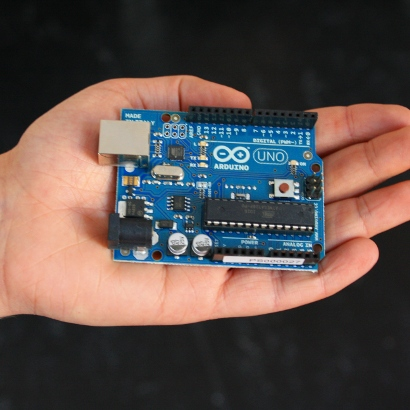
\includegraphics[scale=0.5]{images/arduino_uno_test.jpg} 
   \caption{Placa Arduino Uno}
   \label{fig:example}
\end{figure}


\
\begin{thebibliography}{9}

\bibitem{lamport94}
  Arduino
  
   \url{http://arduino.cc/}

\bibitem{}

\end{thebibliography}

\end{document}
